\chapter{The acoustic landscape of voice quality in Santiago Laxopa Zapotec} \label{ch:acousticlandscape}

%--------------------------------------------------------------------------
\section{Introduction} \label{sec:acousticlandscape:intro}
%--------------------------------------------------------------------------

This chapter details a study of the acoustic dimension of voice quality in Santiago Laxopa Zapotec (SLZ) using a Multidemicensional Scaling (MDS) analysis of acoustic data. MDS is a statistical method of reducing the dimensionality of a dataset to visualize the relationships between the data points. In this study, MDS is used to visualize the acoustic space of voice quality in SLZ. The results of this analysis provide insight into the acoustic correlates of voice quality in SLZ and contribute to our understanding of the phonetic properties of this under-documented language.

This study is based on the work conducted by \citet{keatingCrosslanguageAcousticSpace2023} on the acoustic space of voice quality in 11 languages. However, this study focuses on a single language, SLZ, and provides a detailed analysis of the acoustic properties of voice quality in this language. The results of this study will contribute to our understanding of the phonetic properties of SLZ and  how the acoustic properties of voice quality in this language compare to other languages.

%--------------------------------------------------------------------------
\section{Methods} \label{sec:acousticlandscape:methods}
%--------------------------------------------------------------------------
\subsection{Participants} \label{sec:acousticlandscape:participants}

This study uses data collected from 10 native speakers of SLZ during the summer of 2022. Participants were recruited from the community of Santiago Laxopa, Oaxaca, Mexico. All participants were native speakers of SLZ. Participants were between the ages of 18 and 60 and consisted of 5 males and 5 females.
\subsection{Recordings} \label{sec:acousticlandscape:recordings} 
The participants were asked to perform a word list elicitation task consisting of 76 words. These words were selected to elicit a wide range of voice quality types, including modal, creaky, and breathy voice. The words were selected based on previous research conducted as part of the Zapotec Language Project at the University of California, Santa Cruz \citep{ZapotecLanguageProject}. 
Because participants were not literate in SLZ, the word list was prompted for them by asking them ``How do you say [word in Spanish]?" in Zapotec by myself and another researcher. Participants were asked to respond with the desired word in the carrier phrase \textit{Shnia' [WORD] chonhe lhas} ``I say [WORD] three times.'' which was repeated three times. These utterances were recorded in a quiet environment using a Zoom H4n digital recorder. The recordings were saved as 16-bit WAV files with a sampling rate of 44.1 kHz.

\subsection{Acoustic measuring} \label{sec:acousticlandscape:analysis}
These resulting audio files were then processed in Praat in order to isolate the vowel portion of each word. The vowel onset was set to the second glottal pulse following the onset and the vowel offset was set to the last glottal pulse before the drop in amplitude at the end of the vowel \citep{garellekAcousticDiscriminabilityComplex2020}. The vowel was then extracted and saved as a separate file for analysis.

These vowels were fed into VoiceSauce \citep{shueVOICESAUCEProgramVoice2009} to generate the acoustic measures for the studies discussed in this dissertation. Because many of the acoustic measures are based on the fundamental frequency; this measure was calculated using the STRAIGHT algorithm from \citep{kawaharaInstantaneousfrequencybasedPitchExtraction1998}. The STRAIGHT algorithm estimates the fundamental frequency at one-millisecond (ms) intervals. Once the fundamental frequency is estimated, VoiceSauce then uses an optimization function to locate the harmonics of the spectrum, finding their amplitudes.

VoiceSauce then uses the Snack Sound toolkit \citep{sjolanderSnackSoundToolkit2004} to find the frequencies and bandwidths of the first four formants, also at one-millisecond intervals. The amplitudes of the harmonics nearest to these formant frequencies are located and treated as the amplitudes of the formants. These formant frequencies and bandwidths are used to correct the harmonic amplitudes for the filtering effects of the vocal tract, using \citeauthor{iseliAgeSexVowel2007}'s \citeyear{iseliAgeSexVowel2007} extension of the method employed by \citet{hansonGlottalCharacteristicsFemale1997}. Each vowel was measured across ten equal time intervals, resulting in 22890 data points in total. These measures were then z-scored by speaker to reduce the variation between the speakers and provide a way to directly compare the different measures on the same scale.

\subsection{Data processing} \label{sec:acousticlandscape:processing}
Data points with an absolute z-score value greater than 3 were considered outliers and excluded from the analyses in the dissertation. Within each vowel category, I calculated the Mahalanobis distance in the F1-F2 panel. Each data point with a Mahalanobis distance greater than 6 was considered an outlier and excluded from the analysis.  

Energy was excluded if it had a value of zero and then log-transformed to normalize its right-skewed distribution. Afterward, the resulted log-transformed data was z-scored and any data point with a z-score larger than 3 was excluded. This outlier removal resulted in 1918 datapoints being removed. 

After the outliers were removed, I calculated residual H1* for the remaining data points following \citet{chaiH1H2Acoustic2022}. First, a linear mixed effects model was generated with the z-scored H1* as the response variable and the z-scored energy as fixed effect. The uncorrelated interaction of the z-scored energy by speaker was treated as random. The energy factor resulting from this linear mixed-effects model was extracted. Finally, the z-scored H1* had the product of the z-scored energy and the energy factor subtracted from it.

Once these steps were completed, I took the mean of intervals 5-6 for each vowel and speaker. This is similar to what \citet{keatingCrosslanguageAcousticSpace2023} did by taking the middle of the vowel for their analysis. The reason for this choice is to minimize the effect of the onset and offset of the vowel on the acoustic measures which are more likely to be affected by the surrounding consonants and should give us the most accurate representation of the vowel quality. Because z-scores were used, this resulted in measures that were negative which presents a problem for the MDS analysis. To correct for this, I added the absolute value of the minimum z-score to each measure. This results in a dataset that still preserves the relative differences in the scores while providing a dataset that is all positive for the MDS analysis.


\subsection{Statistical analysis} \label{sec:acousticlandscape:statistics}

Using a multidimensional scaling (MDS) analysis is a statistical method of reducing the dimensionality of a dataset to visualize the relationships between the data points \citep{b.kruskalMultidimensionalScaling1978}. This is especially true when there are many variables that are could contribute to the data. In the case of voice quality this is especially true. As shown in \citet{kreimanUnifiedTheoryVoice2014,kreimanValidatingPsychoacousticModel2021,garellekAcousticDiscriminabilityComplex2020} voice quality is pscyhoacoustically complex and a single measure is not enough to capture the full range of voice quality. Instead what is required is multiple measures that function as cues for the different types of voice quality. For example, a vowel that is characterized as having breathy voice has an elevated spectral-slope and a lowered harmonics-to-noise ratio than modal voice. A creaky voice is characterized as having a lowered spectral-slope and a lowered harmonics-to-noise ratio. 

Because MDS analyses of many variables can result in rather unmeaningful results, I chose to focus on the speaker x voice quality interaction. This is provides us with the opportunity to see how the speakers differ in their production of the different voice qualities. This means that each speakers production of the four phonation contrasts is represented as a single point in the MDS plot. This is similar to what \citet{keatingCrosslanguageAcousticSpace2023} did in their study of the acoustic space of voice quality in 11 languages. Except they compared the language x voice quality interaction. Both of these interactions show us similar information, one shows us within a language while other shows us between languages.

The MDS analysis was conducted in R using the  `metaMDS' function in the `vegan' package. The Manhattan distance was used to estimate the physical differences between the pairs of speaker x voice quality. Because the distances are non-Euclidean, the MDS analysis was conducted using the non-metric option. 

This algorithm resulted in a solution involving a number of different dimensions. The number of dimensions that are retained directly affects how well the original data is captured. To many dimensions and the data is overfit, to few and the data is underfit. To determine the number of dimensions to retain, I used a scree plot to plot the stress of each dimension. The `elbow' of the curve was identified as the correct number of dimensions for the analysis. Figure \ref{fig:stress_plot} shows that the majority of the data can be captured in a two-dimensional space. With the third dimension add some more subtle information about the voice quality.

\begin{figure}[!h]
    \centering
    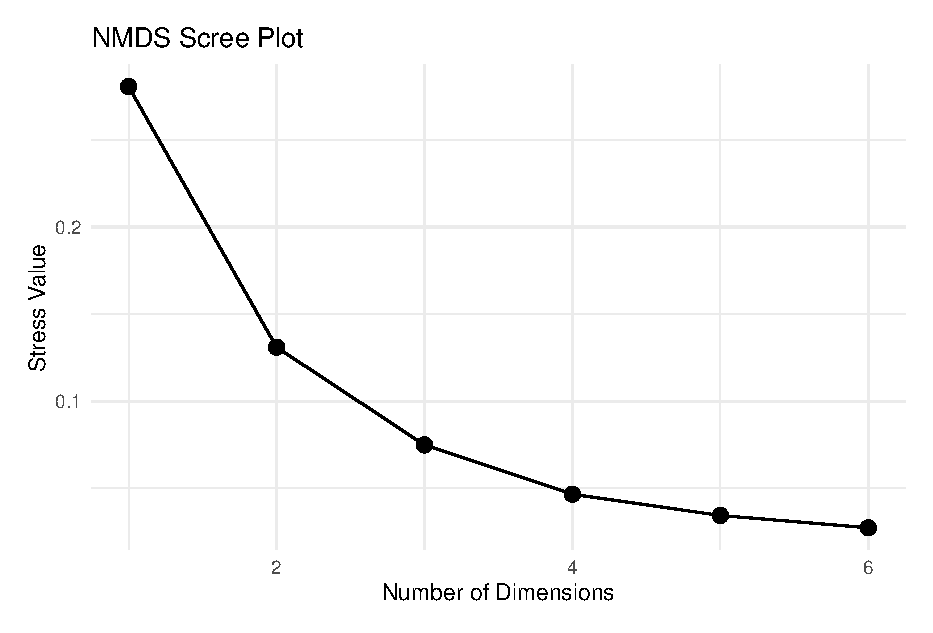
\includegraphics{images/stress_plot.eps}
    \caption{Scree plot for the MDS analysis.}
    \label{fig:stress_plot}
\end{figure}
%--------------------------------------------------------------------------
\section{Results} \label{sec:acousticlandscape:results}
%--------------------------------------------------------------------------
\subsection{Acoustic space of voice quality} \label{sec:acousticlandscape:space}
As mentioned above results of the MDS analysis can be represented in a two-dimensional space, as shown in Figure~\ref{fig:nmds12}. In this and all subsequent plots, breathy voice is represented by black, checked voice with orange, rearticulated voice with green, and modal voice with blue. Overall, we see that breathy voice is located to the left of the plot, checked and rearticulated voice are tending to the right, and modal voice is located in the center along the first dimension. The second dimension shows a modal and nonmodal split with modal voice at the bottom of the plot and nonmodal voice at the top.
\begin{figure}[!h]
    \centering
    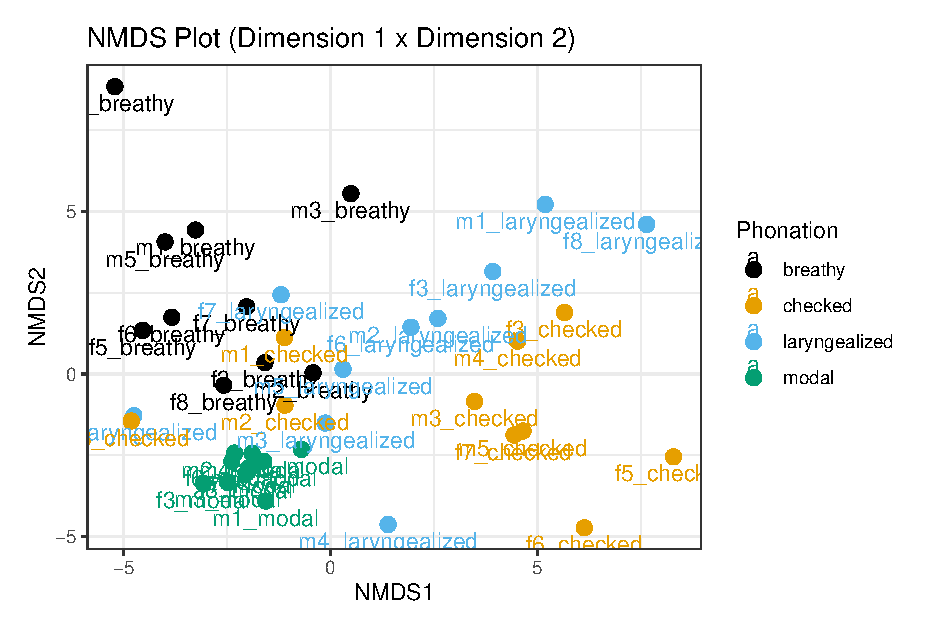
\includegraphics{images/nmds12.eps}
    \caption{Two-dimensional MDS solution showing the first and second dimensions.}
    \label{fig:nmds12}
\end{figure}
    
As mentioned above, the third dimension adds more information about voice quality. The addition of the third dimension helps to spread out the groups along the first dimension, as shown in Figure~\ref{fig:nmds13}. We see that breathy vowels are located at the top of the plot and the two types of creaky voice (checked and rearticulated) are at the bottom of the plot. 

\begin{figure}[!h]
        \centering
        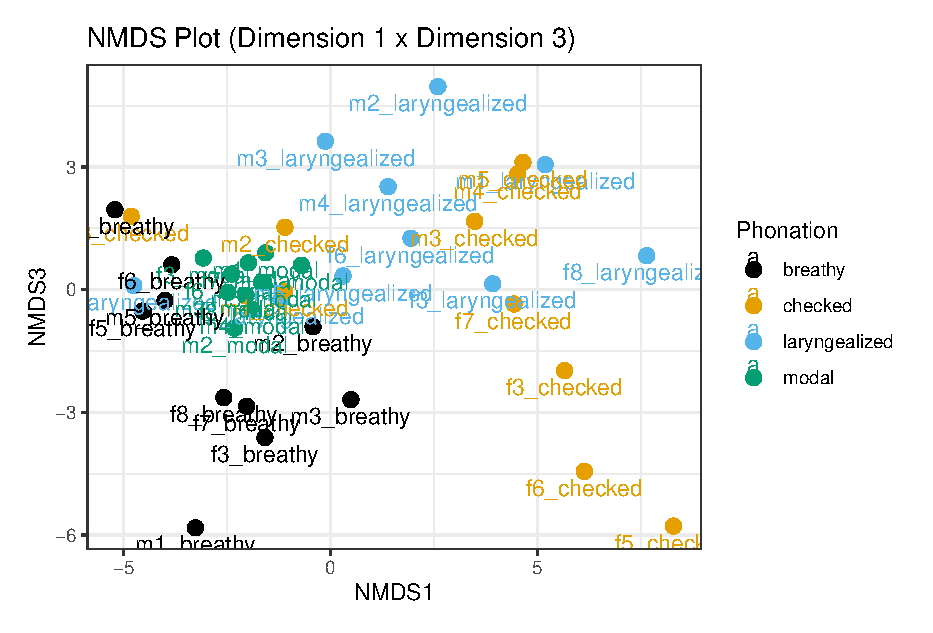
\includegraphics{images/nmds13.eps}
        \caption{Two-dimensional MDS solution showing the first and third dimensions.}
        \label{fig:nmds13}
\end{figure}
    
When the third dimension is added to the second, we see that breathy voices becomes separated from the other nonmodal voice qualities, as shown in Figure~\ref{fig:nmds23}. 

\begin{figure}[!h]
    \centering
    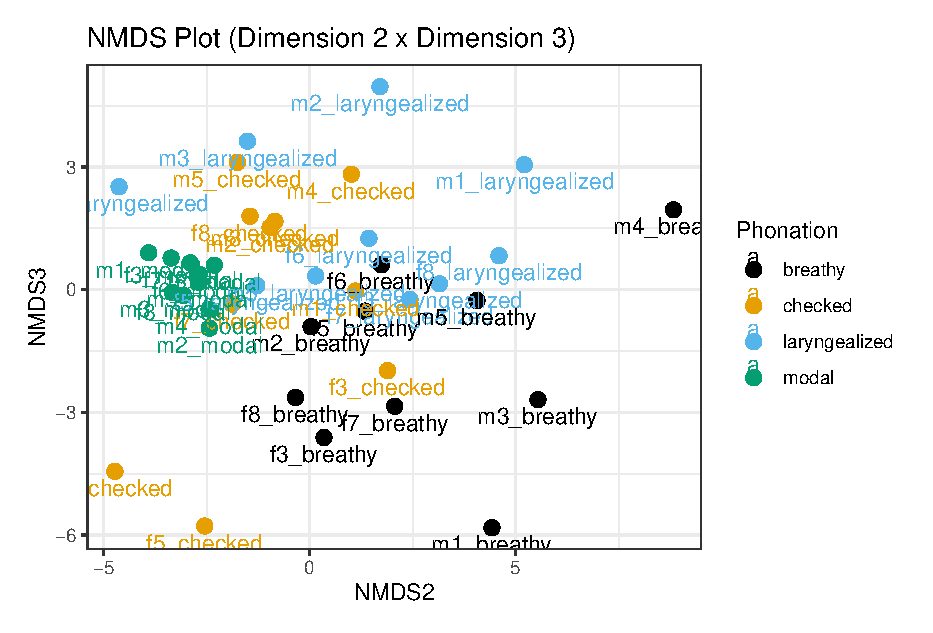
\includegraphics{images/nmds23.eps}
    \caption{Two-dimensional MDS solution showing the second and third dimensions.}
    \label{fig:nmds23}
\end{figure}


\subsection{Acoustic correlates of voice quality} \label{sec:acousticlandscape:correlates}

An additional step to the MDS analysis involves testing which acoustic measures contribute the most weight to the different dimensions. Table~\ref{tab:acoustic_correlates} shows how the 

\begin{table}[ht]
    \centering
    \caption{Weight of each acoustic measure along each dimension of the three-dimensional MDS solution (D1, D2, D3). Parameters that have weights higher than those of other parameters on each dimension are in boldface (weights > 4.0 for D1 and D2, and the weights > 3.0 for D3).} 
    \label{tab:acoustic_correlates}
    \begin{tabular}{lrrr}
    \hline
    Acoustic Measure & D1 & D2 & D3 \\ 
    \hline
    h1h2 & 1.03 & 1.01 & 0.39 \\ 
    h2h4 & 1.15 & 3.98 & 2.13 \\ 
    h1a1 & 2.22 & \textbf{5.15} & 1.84 \\ 
    h1a2 & 2.93 & \textbf{4.66} & 1.00 \\ 
    h1a3 & 2.37 & 3.24 & 0.90 \\ 
    h42k & 1.47 & 0.31 & 1.59 \\ 
    h2kh5k & 3.73 & 0.73 & 0.84 \\ 
    h2 & 1.76 & 0.94 & \textbf{4.09} \\ 
    h4 & 0.79 & 4.28 & 0.10 \\ 
    a1 & \textbf{4.96} & \textbf{5.48} & 0.17 \\ 
    a2 & \textbf{5.30} & \textbf{4.90} & 1.38 \\ 
    a3 & \textbf{4.54} & 2.91 & 1.11 \\ 
    cpp & 4.08 & 0.10 & 1.68 \\ 
    hnr05 & \textbf{5.66} & 1.47 & 1.81 \\ 
    hnr15 & 3.95 & 2.68 & \textbf{3.08} \\ 
    hnr25 & 3.15 & 1.63 & \textbf{3.42} \\ 
    hnr35 & 2.86 & 0.55 & \textbf{3.19} \\ 
    soe & 2.09 & 0.78 & 0.36 \\ 
    shr & 2.39 & 0.50 & 0.47 \\ 
    energy & 2.22 & 3.91 & 0.64 \\ 
    h1\_resid & 1.75 & 0.97 & \textbf{4.24} \\ 
    \hline
    \end{tabular}
\end{table}

%--------------------------------------------------------------------------
\section{Discussion} \label{sec:acousticlandscape:discussion}
%--------------------------------------------------------------------------
